% ==============================================================================
% PLANTILLA DE INFORME -PFM02 /IIIEPE /MAEM
% ==============================================================================
% Uso:
% 1. Duplica este archivo y renombra la copia por unidad, sesion y actividad.
% 2. Actualiza documenttitle, documentsubtitle, documentsubject, sesionname,
%    activityname, docente y fecha de entrega.
% 3. Lee la consigna del EVA/posgrado y NO pegues las instrucciones completas
%    dentro del producto final. Usa la consigna como lista de cumplimiento.
% 4. Revisa la bibliografia indicada, toma notas, registra citas y redacta con
%    comprension propia.
% 5. Identifica el producto academico o didactico solicitado y construyelo dentro
%    del documento siempre que sea posible.
% 6. Entrega en PDF con la nomenclatura indicada por la unidad de aprendizaje.
%
% Formato institucional recomendado para IIIEPE:
% -Fuente tipo Helvetica, equivalente visual a Arial.
% -Interlineado 1.5.
% -Citas autor-anio con natbib: usar \citep{clave} o \citet{clave}.
% -Referencias en bibliografia BibTeX, formato APA 7 en cuerpo y referencias.
% -Caratula, resumen breve, desarrollo, producto solicitado, conclusion y
%   bibliografia.
% -Redaccion academica clara, coherente, cohesionada, formal y sin faltas.
% -Portada con identidad IIIEPE, programa MAEM, matricula y correo institucional.
% -La portada puede llevar una marca de agua institucional discreta; ajustar
%   las variables coverwatermark... si se requiere apagarla o cambiar intensidad.
%
% Criterios generales de cumplimiento:
% -Responder exactamente a la actividad solicitada en el EVA o por la figura docente.
% -Alinear contenido matematico, PDA, aprendizaje de la secuencia, fases,
%   evaluacion y retroalimentacion.
% -Identificar conceptos, elementos, criterios o categorias de forma precisa.
% -Analizar, interpretar y tomar postura; no solo copiar fuentes.
% -Organizar la informacion por jerarquia, secuencia y criterios claros.
% -Incluir conclusion personal cuando la actividad lo permita o lo solicite.
% -Usar citas y referencias en APA 7.
% -Evitar copiar las indicaciones de la actividad en el cuerpo final.
%
% Regla para productos visuales:
% -Si la actividad pide tabla, cuadro comparativo, esquema, mapa conceptual,
%   mapa mental, linea de tiempo, diagrama, matriz, lista de verificacion, red
%   conceptual, SQA, organizador grafico o producto similar, realizarlo
%   preferentemente con LaTeX/TikZ para mantener nitidez, evidencia editable y
%   diseno controlado.
% -Si la consigna exige Canva, Miro u otra herramienta externa, insertar una
%   captura nitida y conservar la explicacion dentro del documento.
% -Para tablas extensas, usar pagina limpia, sin encabezados ni pies, landscape,
%   letra pequena y restaurar el estilo al terminar.
%
% Criterios de redaccion personal:
% -No escribir para llenar espacio; escribir para sostener una idea.
% -Convertir informacion en criterio: que significa, como funciona, que problema
%   resuelve, que limite presenta y que consecuencia produce.
% -Estructura mental recomendada: problema -> sistema -> consecuencia -> postura.
% -Usar pensamiento de diagnostico: entrada -> proceso -> salida.
% -Cada parrafo debe tener funcion: presentar, explicar, comparar, valorar o
%   concluir.
% -Usar primera persona con moderacion academica: "Considero que",
%   "Desde esta perspectiva", "La posicion que sostengo es". Evitar "yo creo".
%
% Notas de enfoque personal segun enfoque_personal.txt:
% -La voz debe ser academica, tecnica, directa, estrategica y funcional.
% -El texto no debe sonar como estudiante pasivo que recopila: debe sonar como
%   alguien que interpreta, ordena, cruza datos y busca consecuencia practica.
% -Antes de redactar, identificar la funcion de cada seccion: abrir problema,
%   definir criterio, demostrar con evidencia, comparar, valorar o concluir.
% -Evitar frases genericas como "es importante porque si" o "desde siempre".
%   Sustituirlas por relaciones verificables: causa, efecto, limite, costo,
%   funcion, riesgo, implicacion o mejora.
% -Cada concepto debe pasar de definicion a analisis. Formula util:
%   concepto -> funcion -> riesgo si se aplica mal -> consecuencia -> postura.
% -La postura personal no debe ser opinion suelta. Debe tener tres piezas:
%   posicion, razon y efecto. Ejemplo: "Considero que X, porque Y; por ello Z".
% -Integrar experiencia o criterio propio sin perder formalidad: no narrar la
%   vida personal, sino usar mirada practica para explicar por que el tema
%   importa en educacion, derecho, instituciones, comunicacion o profesion.
%
% Estilo observado en actividades ya realizadas:
% -Abrir con una tesis concreta:
%   "La ensenanza de las matematicas no solo transmite procedimientos:
%   organiza formas de razonar, representar y justificar."
% -Formular el problema en negativo y positivo:
%   "El problema no es solo..., sino..."
% -Convertir el producto visual en argumento:
%   "El cuadro no solo recopila datos; reconstruye la funcion, el problema y el
%   punto que requiere correccion."
% -Cerrar con aprendizaje transferible:
%   "No basta con saber que dice la norma; tambien debe analizarse a quien
%   protege, a quien excluye y que razones permiten defenderla publicamente."
%
% Nivel cognitivo esperado:
% -Recordar: usar solo para definir conceptos basicos. No debe ser el nivel
%   dominante en una actividad ponderable.
% -Comprender: explicar con palabras propias y relacionar con el tema.
% -Aplicar: llevar el concepto a un caso, norma, texto, correo, dilema o hecho.
% -Analizar: separar elementos, detectar causas, efectos, tensiones y limites.
% -Evaluar: sostener una postura con criterios, fuentes y consecuencias.
% -Crear: elaborar producto propio: mapa, cuadro, linea de tiempo, ensayo,
%   propuesta, reformulacion, glosario, portafolio o solucion argumentada.
%
% Regla de nivel minimo:
% -Si la actividad vale puntos y pide producto, no quedarse en recordar o
%   comprender. Debe llegar por lo menos a aplicar y analizar; si pide conclusion
%   o postura, debe llegar a evaluar.
%
% Uso de tecnicas didacticas:
% -Esta plantilla conserva el manual "Tecnicas didacticas del aprendizaje" como
%   apoyo para construir productos visuales, analiticos y reflexivos.
% -Cuando la actividad mencione una tecnica didactica, identificar: definicion
%   de la tecnica, producto esperado, pasos de construccion, criterios de revision
%   y cierre reflexivo.
% -La tecnica didactica no debe verse como adorno. Debe mostrar seleccion,
%   jerarquia, relacion entre ideas y lectura propia.
% -Siempre que sea viable, construir la tecnica en LaTeX/TikZ: cuadro
%   comparativo, mapa conceptual, esquema, mapa mental, linea de tiempo, matriz,
%   red conceptual, diagrama de flujo, tabla SQA o lista de verificacion.
%
% Checklist antes de entregar:
% [ ] El titulo, unidad de aprendizaje, sesion, docente y fecha estan actualizados.
% [ ] El objetivo coincide con la consigna del EVA/posgrado.
% [ ] El contenido, PDA y aprendizaje de la secuencia estan alineados.
% [ ] La actividad considera las cinco fases de PFM02 cuando se trate de una secuencia.
% [ ] La practica incluye mecanizacion, variacion y al menos una situacion en contexto.
% [ ] La evaluacion mide el aprendizaje declarado y no solo la repeticion del algoritmo.
% [ ] El producto solicitado aparece visible, rotulado y completo.
% [ ] La introduccion plantea un problema o postura, no solo anuncia el tema.
% [ ] El desarrollo explica, conecta y analiza.
% [ ] Hay citas APA autor-anio dentro del texto.
% [ ] La bibliografia final coincide con las fuentes citadas.
% [ ] La conclusion responde que se comprendio y que postura se sostiene.
% [ ] El nivel cognitivo llega al menos a aplicacion y analisis.
% [ ] Si hay conclusion/postura, incluye posicion, razon y consecuencia.
% [ ] La tecnica didactica solicitada esta construida y explicada.
% [ ] No aparecen instrucciones copiadas de la consigna dentro del producto.
% [ ] Ortografia, acentos, sintaxis y nombres propios revisados.
% [ ] Si se uso IA como apoyo, el texto fue comprendido, revisado y apropiado.
% ==============================================================================

% CREACION DEL DOCUMENTO
\documentclass[
	spanish,
	letterpaper, oneside
]{article}

% ==============================================================================
% INFORMACION DEL DOCUMENTO
% Actualizar en cada actividad.
% Ejemplos:
% \def\documenttitle {Cuadro comparativo de conceptos fundamentales}
% \def\documentsubtitle {Actividad X - Nombre de la asignatura}
% \def\documentsubject {Actividad Semana X}
% ==============================================================================
\def\documenttitle {Conversión de fracciones a decimales y viceversa}
\def\documentsubtitle {PFM02 - Temas selectos de matemáticas I}
\def\documentsubject {Sesión 01 -- Secuencia didáctica con solución de actividades}

\def\documentauthor {Mtro. Martín Jonathan de la Cruz Muñoz}
\def\coursename {Temas selectos de matemáticas I}
\def\coursecode {PFM02}

\def\universityname {Instituto de Investigación, Innovación y Estudios de Posgrado \\ para la Educación del Estado de Nuevo León}
\def\universityfaculty {Maestría en Aprendizaje y Enseñanza de las Matemáticas}
\def\universitydepartment {Temas selectos de matemáticas I}
\def\universitydepartmentimage {img/iiiepe/marca-iiiepe.png}
\def\universitydepartmentimagecfg {height=1.75cm}
\def\universitylocation {Monterrey, Nuevo León}

% DATOS FIJOS DEL POSGRADO
\def\studentfullname {Mtro. Martín Jonathan de la Cruz Muñoz}
\def\studentid {00841}
\def\studentemail {martin.delacruz@campus.iiiepe.edu.mx}
\def\institutionurl {https://iiiepe.edu.mx/}
\def\programperiod {1er tetramestre marzo--julio 2026}
\def\programmodality {Modalidad presencial}
\def\programshort {MAEM}
\def\maemsource {https://iiiepe.edu.mx/maestria-en-aprendizaje-y-ensenanza-de-las-matematicas/}
\def\coursegroup {Grupo A}
\def\courseperiod {Marzo--julio 2026}
\def\evaname {EVA posgrado}
\def\activityname {S01 -- Conversión de fracciones a decimales y viceversa}
\def\sessionname {Sesión 01}
\def\blockname {Bloque 1: Números racionales y sus representaciones}
\def\methodology {Aprendizaje basado en indagación}
\def\steamenfoque {STEAM como enfoque}
\def\curriculumsource {Programa Sintético Fase 6}
\def\formativefield {Saberes y Pensamiento Científico}
\def\mainproduct {Informe académico con secuencia didáctica matemática}
\def\docentename {Mtro. Jonathan Cárdenas (Coordinador PFM02)}

% INTEGRANTES, PROFESORES Y FECHAS
\def\authortable {
	\begin{tabular}{ll}
		\textbf{Alumno:}
		& \begin{tabular}[t]{l}
			 \studentfullname \\
		\end{tabular} \\
		Matricula: & \studentid \\
		Correo institucional: & \studentemail \\

		\textit{Figura docente:}
		& \begin{tabular}[t]{l}
			\docentename
		\end{tabular} \\
		Unidad: & \coursename \\
		Clave: & \coursecode \\
		Grupo: & \coursegroup \\
		Sesión/Bloque: & \sessionname\ / \blockname \\
		Actividad: & \activityname \\
		Programa: & \programshort \\
		Periodo: & \courseperiod \\
		& \\
		\multicolumn{2}{l}{Fecha de realizacion: \today} \\
		\multicolumn{2}{l}{\universitylocation}
	\end{tabular}
}

% IMPORTACION DEL TEMPLATE BASE
\input{template}

% FORMATO GENERAL
\usepackage{helvet}
\renewcommand{\familydefault}{\sfdefault}

% IDENTIDAD VISUAL IIIEPE
\definecolor{iiiepeNavy}{HTML}{163B5C}
\definecolor{iiiepeBlue}{HTML}{1F6F9F}
\definecolor{iiiepeAqua}{HTML}{20B7A8}
\definecolor{iiiepeOrange}{HTML}{F28C28}
\definecolor{iiiepePaper}{HTML}{F6F8F7}
\definecolor{iiiepeInk}{HTML}{1E2A32}
\definecolor{iiiepeMuted}{HTML}{667085}
\def\portraittitlecolor {iiiepeNavy}

% TABLAS Y PRODUCTOS VISUALES
\usepackage{array}
\usepackage{tabularx}
\usepackage{makecell}
\usepackage{longtable}
\usepackage{etoolbox}
\usepackage{pdflscape}
\usepackage{graphicx}
\usepackage{float}
\usepackage{tikz}
\setlength{\LTcapwidth}{\textwidth}
\newcommand{\PFMTableSetup}{%
	\small
	\renewcommand{\arraystretch}{1.35}%
	\setlength{\tabcolsep}{4pt}%
	\rowcolors{2}{gray!10}{white}%
}
\AtBeginEnvironment{longtable}{\PFMTableSetup}
\AtEndEnvironment{longtable}{\rowcolors{2}{}{}}
\usetikzlibrary{
	arrows.meta,
	positioning,
	calc,
	matrix,
	fit,
	shapes.geometric,
	shapes.callouts,
	decorations.pathreplacing,
	backgrounds,
	shadows.blur
}

\tikzset{
	paso/.style={
		draw=iiiepeBlue,
		rounded corners=2mm,
		fill=iiiepeBlue!8,
		align=center,
		inner sep=5pt,
		font=\small
	},
	dato/.style={
		draw=iiiepeNavy,
		rounded corners=2mm,
		fill=iiiepePaper,
		align=center,
		inner sep=5pt,
		font=\small\bfseries
	},
	resultado/.style={
		draw=iiiepeAqua!80!black,
		rounded corners=2mm,
		fill=iiiepeAqua!12,
		align=center,
		inner sep=5pt,
		font=\small\bfseries
	},
	verificacion/.style={
		draw=iiiepeOrange,
		rounded corners=2mm,
		fill=iiiepeOrange!12,
		align=center,
		inner sep=5pt,
		font=\scriptsize
	},
	nota/.style={
		draw=iiiepeOrange,
		rounded corners=2mm,
		fill=iiiepeOrange!10,
		align=center,
		inner sep=4pt,
		font=\scriptsize
	},
	flecha/.style={
		-{Latex[length=2.5mm]},
		thick,
		iiiepeBlue
	},
	flechaSecundaria/.style={
		-{Latex[length=2.2mm]},
		thick,
		dashed,
		iiiepeOrange
	},
	resaltar/.style={
		draw=iiiepeOrange,
		rounded corners=1.5mm,
		thick,
		inner sep=2pt
	}
}

\newcommand{\cadenaConversion}[4]{%
\begin{tikzpicture}[node distance=1.25cm]
	\node[dato] (a) {#1};
	\node[paso, right=of a] (b) {#2};
	\node[resultado, right=of b] (c) {#3};
	\node[verificacion, below=0.65cm of b] (d) {#4};
	\draw[flecha] (a) -- (b);
	\draw[flecha] (b) -- (c);
	\draw[flechaSecundaria] (d) -- (b);
\end{tikzpicture}%
}

\newcommand{\ejercicioTikzTresPasos}[5]{%
\begin{tikzpicture}[node distance=0.95cm and 1.1cm]
	\node[dato] (dato) {#1};
	\node[paso, right=of dato] (puno) {#2};
	\node[paso, right=of puno] (pdos) {#3};
	\node[resultado, right=of pdos] (res) {#4};
	\node[verificacion, below=0.75cm of pdos] (ver) {#5};
	\draw[flecha] (dato) -- (puno);
	\draw[flecha] (puno) -- (pdos);
	\draw[flecha] (pdos) -- (res);
	\draw[flechaSecundaria] (ver) -- (pdos);
\end{tikzpicture}%
}

\newcommand{\DivOp}[2]{\ensuremath{#1\,\mbox{ entre }\,#2}}

% CITAS EN FORMATO AUTOR-ANIO, COMPATIBLE CON APA 7 EN EL CUERPO DEL TEXTO
% Usar:
% - Cita parentetica: \citep{clave}
% - Cita narrativa: \citet{clave}
% - Varias fuentes: \citep{clave1,clave2}
\setcitestyle{authoryear,open={(},close={)}}

% ==============================================================================
% AYUDAS DE REDACCION
% Quitar o comentar \pendiente cuando el documento final este terminado.
% ==============================================================================
\newcommand{\pendiente}[1]{\textcolor{red}{[PENDIENTE: #1]}}

% ==============================================================================
% MARCA DE AGUA EN PORTADA
% - Se aplica solo a la portada porque usa \AddToShipoutPictureBG*.
% - Para apagarla en alguna actividad: \def\coverwatermarkenabled {false}
% - Usar opacidad baja para que no compita con titulo, datos ni logotipo.
% ==============================================================================
\def\coverwatermarkenabled {true}
\def\coverwatermarkimage {img/iiiepe/logo-puntos.png}
\def\coverwatermarkopacity {0.09}
\def\coverwatermarkwidth {0.58\paperwidth}
\def\coverwatermarkxshift {0cm}
\def\coverwatermarkyshift {-0.15cm}

\newcommand{\insertcoverwatermark}{%
	\ifthenelse{\equal{\coverwatermarkenabled}{true}}{%
		\AddToShipoutPictureBG*{%
			\begin{tikzpicture}[remember picture,overlay]
				\node[
					opacity=\coverwatermarkopacity,
					inner sep=0pt,
					xshift=\coverwatermarkxshift,
					yshift=\coverwatermarkyshift
				] at (current page.center) {%
					\includegraphics[width=\coverwatermarkwidth]{\coverwatermarkimage}%
				};
			\end{tikzpicture}%
		}%
	}{}%
}

\begin{document}

% PORTADA
\insertcoverwatermark
\templatePortrait

% CONFIGURACION DE PAGINA Y ENCABEZADOS
\templatePagecfg
\onehalfspacing

% ==============================================================================
% RESUMEN / ABSTRACT
% Debe ser breve. Fórmula recomendada:
% Tema + objetivo + técnica/producto + enfoque personal.
% ==============================================================================
\begin{abstractd}
	\textbf{Objetivo:} Resolver y mejorar la actividad de la Sesión 01 sobre conversión de fracciones a decimales y de decimales a fracciones, incorporando retroalimentación derivada del trabajo posterior con la Sesión 02.

	\textbf{Contenido:} Expresión de fracciones como decimales y de decimales como fracciones.

	\textbf{PDA:} Usa diversas estrategias al convertir números fraccionarios a decimales y viceversa.

	\textbf{Aprendizaje de la secuencia:} Convertir fracciones a decimales y viceversa, distinguiendo decimales finitos y periódicos.

	\textbf{Producto:} Reporte académico con procedimientos explícitos, ejercicios resueltos, situaciones contextualizadas, autoevaluación y retroalimentación.
\end{abstractd}

% TABLA DE CONTENIDOS - ÍNDICE
\templateIndex

% CONFIGURACIONES FINALES
\templateFinalcfg

% ======================= INICIO DEL DOCUMENTO =======================

% ==============================================================================
% SECCIÓN 1: INTRODUCCIÓN
% Apertura recomendada:
% - Iniciar con una afirmacion clara, no con una frase generica.
% - Traducir la consigna a un problema academico, didactico, matematico,
%   pedagogico o profesional, segun la unidad de aprendizaje.
% - Explicar por que importa.
% - Cerrar anticipando el enfoque personal.
% ==============================================================================
\section{Introducción}

La conversión entre fracciones y decimales no consiste solo en cambiar la escritura de un número racional: exige reconocer que una misma cantidad puede representarse por valor posicional, división, equivalencia o eliminación del período. Por ello, el procedimiento debe mostrar qué se hace, por qué funciona y cómo se comprueba que la cantidad no cambió.

La retroalimentación obtenida al actualizar la Sesión 02 mostró la necesidad de fortalecer esta actividad con una estructura didáctica más visible: antecedente, explicación, práctica, evaluación y retroalimentación. En consecuencia, la Sesión 01 se reorganiza para que las respuestas no aparezcan como resultados aislados, sino como evidencias de razonamiento matemático.

El propósito de la secuencia es que el estudiante distinga cuándo un decimal es finito, cuándo es periódico, qué estrategia conviene usar en cada caso y cómo verificar el resultado. Así, el aprendizaje se vuelve transferible a medidas, porcentajes, perímetros, edades y situaciones de comparación numérica.

% ==============================================================================
% SECCIÓN 2: DESARROLLO / ANÁLISIS
% Adaptar los subtítulos según la unidad de aprendizaje y la consigna.
%
% Productos posibles:
% - Cuadro comparativo: criterios, evidencia, diferencia, valoracion.
% - Mapa conceptual: concepto central, conceptos secundarios, conectores claros.
% - Línea de tiempo: fecha/etapa, hecho, aporte, consecuencia.
% - Secuencia didáctica: contenido, PDA, fase, actividad, evidencia y evaluación.
% - Estudio de caso: situación, elementos, problema, interpretación, solución.
% - Lista de verificación: criterio observable, indicador, cumplimiento, mejora.
% - Glosario: concepto, definición, función, ejemplo, fuente.
% - Reporte o ensayo: tesis, argumentos, evidencia, postura y cierre.
%
% Regla de párrafo:
% Entrada: concepto o problema.
% Proceso: explicación, fuente y relación.
% Salida: consecuencia, criterio o postura.
% ==============================================================================
\section{Desarrollo de la actividad}

\subsection{Datos de la secuencia}

\begin{longtable}{@{}p{0.28\linewidth}p{0.65\linewidth}@{}}
	\caption{Datos base de la Sesión 01}\label{tab:datos-sesion}\\
	\toprule
	\textbf{Elemento} & \textbf{Descripción} \\
	\midrule
	\endfirsthead
	\toprule
	\textbf{Elemento} & \textbf{Descripción} \\
	\midrule
	\endhead
	Tema & Conversión de fracciones a decimales y viceversa. \\
	Contenido & Expresión de fracciones como decimales y de decimales como fracciones. \\
	Proceso de desarrollo de aprendizaje & Usa diversas estrategias al convertir números fraccionarios a decimales y viceversa. \\
	Aprendizaje de la secuencia & Convertir fracciones a decimales y viceversa. \\
	Producto esperado & Procedimientos escritos, ejercicios resueltos, situaciones en contexto, autoevaluación y retroalimentación. \\
	\bottomrule
\end{longtable}

\subsection{Criterios institucionales incorporados}

\begin{longtable}{@{}p{0.26\linewidth}p{0.32\linewidth}p{0.34\linewidth}@{}}
	\caption{Traducción de criterios institucionales al producto mejorado}\label{tab:criterios-institucionales-s01}\\
	\toprule
	\textbf{Fuente institucional} & \textbf{Criterio recuperado} & \textbf{Aplicación en este reporte y presentación} \\
	\midrule
	\endfirsthead
	\toprule
	\textbf{Fuente institucional} & \textbf{Criterio recuperado} & \textbf{Aplicación en este reporte y presentación} \\
	\midrule
	\endhead
	Estructura de una secuencia didáctica & Cinco fases: antecedente, explicación, práctica, evaluación y retroalimentación. & La actividad inicia con saberes previos, explica rutas de conversión, practica con ejercicios graduados, evalúa en contexto y cierra con criterios de mejora. \\
	Criterios de evaluación & Actividades diarias, exposición de secuencia, escrito reflexivo y exposición final. & El producto deja evidencias observables: estrategia elegida, desarrollo, resultado, simplificación, verificación e interpretación contextual. \\
	Lineamientos de mejora & Cada procedimiento debe mostrar estrategia, desarrollo, resultado y verificación. & Los ejercicios resueltos y situaciones se presentan como procedimientos guiados, no como banco de respuestas aislado. \\
	\bottomrule
\end{longtable}

\subsection{Secuencia didáctica propuesta}

\begin{longtable}{@{}p{0.12\linewidth}p{0.20\linewidth}p{0.35\linewidth}p{0.25\linewidth}@{}}
	\caption{Organización didáctica en cinco fases para la Sesión 01}\label{tab:fases-sesion01}\\
	\toprule
	\textbf{Fase} & \textbf{Función} & \textbf{Actividad matemática} & \textbf{Evidencia} \\
	\midrule
	\endfirsthead
	\toprule
	\textbf{Fase} & \textbf{Función} & \textbf{Actividad matemática} & \textbf{Evidencia} \\
	\midrule
	\endhead
	1 & Antecedente & Recuperar valor posicional, fracciones equivalentes, división y simplificación. & Explicación breve de conceptos base y ejemplos iniciales. \\
	2 & Explicación & Distinguir fracciones decimales, no decimales, decimales finitos y periódicos. & Mapa de decisión y procedimientos con esquemas. \\
	3 & Práctica & Resolver conversiones de fracciones a decimales y de decimales a fracciones. & Tablas con procedimiento y resultado simplificado. \\
	4 & Evaluación & Resolver situaciones en contexto donde la conversión sea necesaria para interpretar una medida o cantidad. & Planteamiento, conversión, respuesta y verificación contextual. \\
	5 & Retroalimentación & Revisar errores frecuentes: dividir al revés, omitir simplificación, no marcar período o perder equivalencia. & Autoevaluación y lista de mejora. \\
	\bottomrule
\end{longtable}

\subsection{Toma de nota}

Una \textbf{fracción decimal} es aquella cuyo denominador es $10$, $100$, $1000$, $10000$, etc. Para convertirla a decimal, se toma el numerador y se cuentan hacia la izquierda tantas cifras decimales como ceros tenga el denominador. Por ejemplo:
\[
	\frac{375}{1000}=0{.}375
\]

Cuando la fracción no tiene denominador decimal, se efectúa la división del numerador entre el denominador. Si el residuo llega a cero, el decimal es finito; si los residuos se repiten, el decimal es periódico. Por ejemplo:
\[
	\frac{8}{11}=0{.}\overline{72}
\]

Para convertir un decimal finito a fracción, se escribe el número sin punto decimal como numerador y como denominador se coloca $1$ seguido de tantos ceros como cifras decimales tenga el número. Después se simplifica:
\[
	4{.}325=\frac{4325}{1000}=\frac{173}{40}
\]

Para convertir un decimal periódico a fracción, se multiplica por potencias de $10$ hasta alinear el período, se restan las expresiones y se despeja la fracción.

\subsection{Procedimientos con esquemas}

Los diagramas siguientes resumen las rutas de conversión y muestran cómo justificar cada procedimiento. Su función es apoyar la comprensión visual del valor posicional, la división y la equivalencia entre representaciones.

\begin{figure}[H]
	\centering
	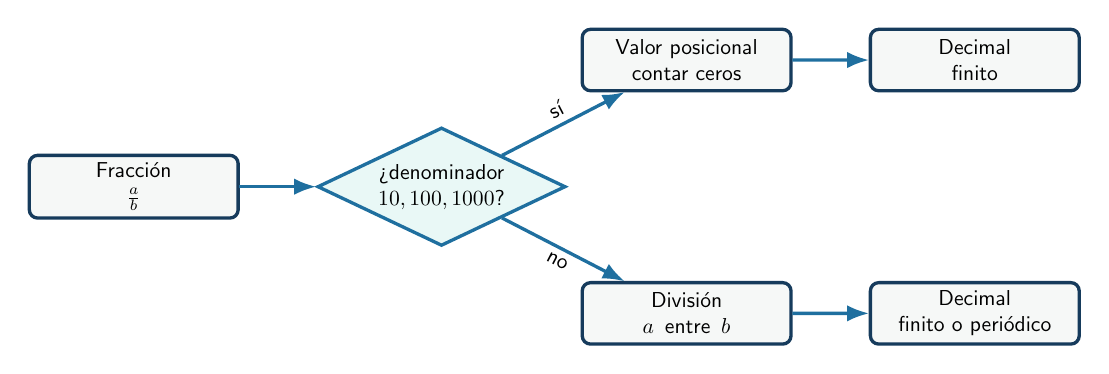
\begin{tikzpicture}[scale=0.78, transform shape,
		node distance=1.05cm and 1.25cm,
		box/.style={rectangle, rounded corners=3pt, draw=iiiepeNavy, very thick, fill=iiiepePaper, align=center, minimum width=3.4cm, minimum height=1cm},
		decision/.style={diamond, aspect=2.1, draw=iiiepeBlue, very thick, fill=iiiepeAqua!10, align=center, inner sep=2pt},
		arrow/.style={-{Latex[length=2.8mm]}, very thick, draw=iiiepeBlue}
	]
		\node[box] (frac) {Fracción\\$\frac{a}{b}$};
		\node[decision, right=of frac] (tipo) {¿denominador\\$10,100,1000$?};
		\node[box, above right=of tipo] (pos) {Valor posicional\\contar ceros};
		\node[box, below right=of tipo] (div) {División\\$\DivOp{a}{b}$};
		\node[box, right=of pos] (finito) {Decimal\\finito};
		\node[box, right=of div] (periodico) {Decimal\\finito o periódico};
		\draw[arrow] (frac) -- (tipo);
		\draw[arrow] (tipo) -- node[above,sloped]{sí} (pos);
		\draw[arrow] (tipo) -- node[below,sloped]{no} (div);
		\draw[arrow] (pos) -- (finito);
		\draw[arrow] (div) -- (periodico);
	\end{tikzpicture}
	\caption{Mapa general para convertir fracciones a decimales.}
\end{figure}

\subsubsection*{Caso 1: fracción decimal}

Cuando el denominador es $10$, $100$, $1000$, etc., el denominador indica la posición decimal. En $\frac{375}{1000}$, el denominador tiene tres ceros; por ello, el punto decimal se coloca tres lugares desde la derecha:
\[
	\frac{375}{1000}=0{.}375
\]

\begin{figure}[H]
	\centering
	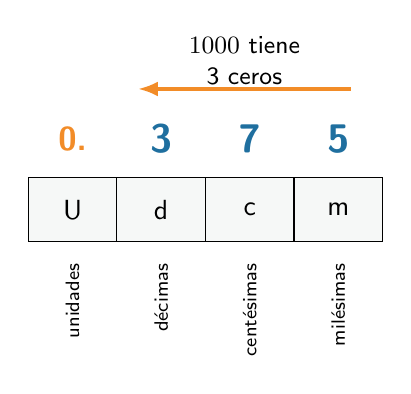
\begin{tikzpicture}[scale=0.9]
		
		% Celdas de valor posicional
		\foreach \x/\lab in {0/U,1/d,2/c,3/m}{
			\draw[fill=iiiepePaper] (\x*1.25,0) rectangle ++(1.25,0.9);
			\node at (\x*1.25+0.625,0.45) {\lab};
		}
		
		% Etiquetas verticales
		\node[font=\scriptsize, rotate=90, anchor=east] at (0.625,-0.18) {unidades};
		\node[font=\scriptsize, rotate=90, anchor=east] at (1.875,-0.18) {décimas};
		\node[font=\scriptsize, rotate=90, anchor=east] at (3.125,-0.18) {centésimas};
		\node[font=\scriptsize, rotate=90, anchor=east] at (4.375,-0.18) {milésimas};
		
		% Número decimal
		\node[font=\large\bfseries, color=iiiepeOrange] at (0.625,1.45) {0.};
		\node[font=\Large\bfseries, color=iiiepeBlue] at (1.875,1.45) {3};
		\node[font=\Large\bfseries, color=iiiepeBlue] at (3.125,1.45) {7};
		\node[font=\Large\bfseries, color=iiiepeBlue] at (4.375,1.45) {5};
		
		% Flecha explicativa
		\draw[-{Latex[length=2.5mm]}, very thick, iiiepeOrange] 
			(4.55,2.15) -- (1.55,2.15);
			
		\node[font=\small, align=center] at (3.05,2.55) 
			{$1000$ tiene\\3 ceros};
		
	\end{tikzpicture}
	\caption{Valor posicional para convertir $\frac{375}{1000}$ en $0.375$.}
\end{figure}

\subsubsection*{Caso 2: fracción no decimal}

Cuando el denominador no es decimal, se divide el numerador entre el denominador. El resultado debe revisarse con una estimación previa: si el numerador es menor que el denominador, el decimal debe ser menor que $1$.

\[
\frac{41}{50}=\DivOp{41}{50}=0{.}82
\]

\[
\begin{array}{rcl}
	\DivOp{41{.}00}{50} &=& 0{.}82\\
	50\times 0{.}8 &=& 40\\
	41-40 &=& 1\\
	\DivOp{1{.}00}{50} &=& 0{.}02
\end{array}
\qquad
0{.}82=\frac{82}{100}=\frac{41}{50}
\]

\subsubsection*{Representación visual de equivalencia}

El siguiente esquema muestra que $\frac{3}{4}$, $\frac{75}{100}$ y $0{.}75$ representan la misma cantidad. Esta representación ayuda a evitar el error de leer $\frac{3}{4}$ como si fuera $0{.}34$.

\begin{figure}[H]
	\centering
	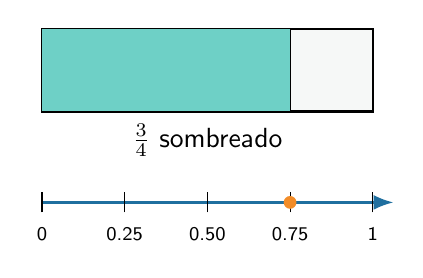
\begin{tikzpicture}[scale=1.05]
		\draw[fill=iiiepePaper, thick] (0,0) rectangle (4,1);
		\foreach \x in {1,2,3}{\draw[thick] (\x,0) -- (\x,1);}
		\fill[iiiepeAqua!65] (0,0) rectangle (3,1);
		\node at (2,-0.35) {$\frac{3}{4}$ sombreado};
		\draw[-{Latex[length=2.5mm]}, thick, iiiepeBlue] (0,-1.1) -- (4.25,-1.1);
		\foreach \x/\lab in {0/0,1/{0{.}25},2/{0{.}50},3/{0{.}75},4/1}{
			\draw (\x,-1.22) -- (\x,-0.98);
			\node[font=\scriptsize] at (\x,-1.48) {\lab};
		}
		\fill[iiiepeOrange] (3,-1.1) circle (2.2pt);
	\end{tikzpicture}
	\caption{Equivalencia visual entre $\frac{3}{4}$ y $0{.}75$.}
\end{figure}

\subsubsection*{Decimal periódico a fracción}

Para un decimal periódico se multiplica por una potencia de $10$ que haga coincidir el período; después se restan las ecuaciones para eliminar la parte infinita.

\[
	x=0{.}181818\ldots
\]
\[
	100x=18{.}181818\ldots
\]
\[
	100x-x=18{.}181818\ldots-0{.}181818\ldots
\]
\[
	99x=18 \qquad x=\frac{18}{99}=\frac{2}{11}
\]

En un decimal periódico mixto, como $0{.}82\overline{1}=0{.}821111\ldots$, se alinean dos expresiones: una antes del período y otra después de la primera repetición.

\[
	x=0{.}821111\ldots
\]
\[
	1000x=821{.}111\ldots \qquad 100x=82{.}111\ldots
\]
\[
	1000x-100x=821{.}111\ldots-82{.}111\ldots
\]
\[
	900x=739 \qquad x=\frac{739}{900}
\]

\section{Ejercicios de práctica}

\subsection{Fracciones decimales a número decimal}

La tabla presenta varios incisos resueltos; el esquema posterior muestra la ruta de procedimiento que se aplica al bloque completo.

\begin{longtable}{@{}p{0.23\linewidth}p{0.23\linewidth}p{0.23\linewidth}p{0.23\linewidth}@{}}
	\caption{Conversión de fracciones decimales}\label{tab:fracciones-decimales}\\
	\toprule
	\textbf{a--e} & \textbf{f--j} & \textbf{k--o} & \textbf{p--t} \\
	\midrule
	\endfirsthead
	\toprule
	\textbf{a--e} & \textbf{f--j} & \textbf{k--o} & \textbf{p--t} \\
	\midrule
	\endhead
	a. $\frac{3}{10}=0{.}3$ & f. $\frac{75}{100}=0{.}75$ & k. $\frac{125}{1000}=0{.}125$ & p. $\frac{45}{1000}=0{.}045$ \\
	b. $\frac{8}{10}=0{.}8$ & g. $\frac{25}{100}=0{.}25$ & l. $\frac{375}{1000}=0{.}375$ & q. $\frac{4}{100}=0{.}04$ \\
	c. $\frac{1}{10}=0{.}1$ & h. $\frac{80}{100}=0{.}80$ & m. $\frac{700}{1000}=0{.}700$ & r. $\frac{815}{10}=81{.}5$ \\
	d. $\frac{6}{10}=0{.}6$ & i. $\frac{50}{100}=0{.}50$ & n. $\frac{615}{1000}=0{.}615$ & s. $\frac{1}{1000}=0{.}001$ \\
	e. $\frac{17}{10}=1{.}7$ & j. $\frac{375}{100}=3{.}75$ & o. $\frac{4455}{1000}=4{.}455$ & t. $\frac{5}{100}=0{.}05$ \\
	\bottomrule
\end{longtable}

\begin{figure}[H]
	\centering
	\resizebox{0.86\linewidth}{!}{%
		\cadenaConversion
			{$\frac{375}{1000}$}
			{Tres ceros $\Rightarrow$ tres cifras decimales}
			{$0{.}375$}
			{El denominador indica el valor posicional.}
	}
	\caption{Procedimiento visual para convertir una fracción decimal a número decimal.}
\end{figure}

\subsection{Fracciones propias a número decimal}

La tabla presenta varios incisos resueltos; el esquema posterior muestra la ruta de procedimiento que se aplica al bloque completo.

\begin{longtable}{@{}p{0.23\linewidth}p{0.23\linewidth}p{0.23\linewidth}p{0.23\linewidth}@{}}
	\caption{Conversión de fracciones propias}\label{tab:fracciones-propias}\\
	\toprule
	\textbf{a--b} & \textbf{c--d} & \textbf{e--f} & \textbf{g--h} \\
	\midrule
	\endfirsthead
	\toprule
	\textbf{a--b} & \textbf{c--d} & \textbf{e--f} & \textbf{g--h} \\
	\midrule
	\endhead
	a. $\frac{3}{4}=0{.}75$ & c. $\frac{1}{8}=0{.}125$ & e. $\frac{5}{16}=0{.}3125$ & g. $\frac{4}{25}=0{.}16$ \\
	b. $\frac{4}{5}=0{.}8$ & d. $\frac{3}{10}=0{.}3$ & f. $\frac{4}{8}=0{.}5$ & h. $\frac{18}{50}=0{.}36$ \\
	\bottomrule
\end{longtable}

\begin{figure}[H]
	\centering
	\resizebox{0.76\linewidth}{!}{%
		\cadenaConversion
			{$\frac{5}{16}$}
			{\DivOp{5}{16}}
			{$0{.}3125$}
			{Como $5<16$, el resultado es menor que $1$.}
	}
	\caption{Procedimiento visual para convertir una fracción propia a decimal.}
\end{figure}

\subsection{Fracciones impropias a número decimal}

La tabla presenta varios incisos resueltos; el esquema posterior muestra la ruta de procedimiento que se aplica al bloque completo.

\begin{longtable}{@{}p{0.23\linewidth}p{0.23\linewidth}p{0.23\linewidth}p{0.23\linewidth}@{}}
	\caption{Conversión de fracciones impropias}\label{tab:fracciones-impropias}\\
	\toprule
	\textbf{a--b} & \textbf{c--d} & \textbf{e--f} & \textbf{g--h} \\
	\midrule
	\endfirsthead
	\toprule
	\textbf{a--b} & \textbf{c--d} & \textbf{e--f} & \textbf{g--h} \\
	\midrule
	\endhead
	a. $\frac{6}{4}=1{.}5$ & c. $\frac{13}{8}=1{.}625$ & e. $\frac{21}{6}=3{.}5$ & g. $\frac{23}{20}=1{.}15$ \\
	b. $\frac{8}{5}=1{.}6$ & d. $\frac{10}{4}=2{.}5$ & f. $\frac{17}{4}=4{.}25$ & h. $\frac{34}{5}=6{.}8$ \\
	\bottomrule
\end{longtable}

\begin{figure}[H]
	\centering
	\resizebox{0.76\linewidth}{!}{%
		\cadenaConversion
			{$\frac{21}{6}$}
			{\DivOp{21}{6}}
			{$3{.}5$}
			{Como $21>6$, el resultado es mayor que $1$.}
	}
	\caption{Procedimiento visual para convertir una fracción impropia a decimal.}
\end{figure}

\subsection{Fracciones mixtas a número decimal}

La tabla presenta varios incisos resueltos; el esquema posterior muestra la ruta de procedimiento que se aplica al bloque completo.

\begin{longtable}{@{}p{0.23\linewidth}p{0.23\linewidth}p{0.23\linewidth}p{0.23\linewidth}@{}}
	\caption{Conversión de fracciones mixtas}\label{tab:fracciones-mixtas}\\
	\toprule
	\textbf{a--b} & \textbf{c--d} & \textbf{e--f} & \textbf{g--h} \\
	\midrule
	\endfirsthead
	\toprule
	\textbf{a--b} & \textbf{c--d} & \textbf{e--f} & \textbf{g--h} \\
	\midrule
	\endhead
	a. $7\frac{2}{5}=7{.}4$ & c. $12\frac{17}{20}=12{.}85$ & e. $5\frac{7}{8}=5{.}875$ & g. $2\frac{8}{5}=3{.}6$ \\
	b. $3\frac{1}{4}=3{.}25$ & d. $1\frac{9}{10}=1{.}9$ & f. $6\frac{13}{40}=6{.}325$ & h. $4\frac{10}{8}=5{.}25$ \\
	\bottomrule
\end{longtable}

\begin{figure}[H]
	\centering
	\resizebox{0.86\linewidth}{!}{%
		\cadenaConversion
			{$6\frac{13}{40}$}
			{$6+\frac{13}{40}$}
			{$6{.}325$}
			{La parte entera se conserva y solo se convierte la fracción.}
	}
	\caption{Procedimiento visual para convertir una fracción mixta a decimal.}
\end{figure}

\subsection{Fracciones no decimales a número decimal}

La tabla presenta varios incisos resueltos; el esquema posterior muestra la ruta de procedimiento que se aplica al bloque completo.

\begin{longtable}{@{}p{0.23\linewidth}p{0.23\linewidth}p{0.23\linewidth}p{0.23\linewidth}@{}}
	\caption{Conversión de fracciones no decimales}\label{tab:fracciones-no-decimales}\\
	\toprule
	\textbf{a--b} & \textbf{c--d} & \textbf{e--f} & \textbf{g--h} \\
	\midrule
	\endfirsthead
	\toprule
	\textbf{a--b} & \textbf{c--d} & \textbf{e--f} & \textbf{g--h} \\
	\midrule
	\endhead
	a. $\frac{1}{3}=0{.}\overline{3}$ & c. $2\frac{7}{11}=2{.}\overline{63}$ & e. $5\frac{4}{15}=5{.}2\overline{6}$ & g. $\frac{6}{27}=0{.}\overline{2}$ \\
	b. $\frac{7}{9}=0{.}\overline{7}$ & d. $\frac{13}{6}=2{.}1\overline{6}$ & f. $\frac{20}{11}=1{.}\overline{81}$ & h. $\frac{22}{90}=0{.}2\overline{4}$ \\
	\bottomrule
\end{longtable}

\begin{figure}[H]
	\centering
	\resizebox{0.82\linewidth}{!}{%
	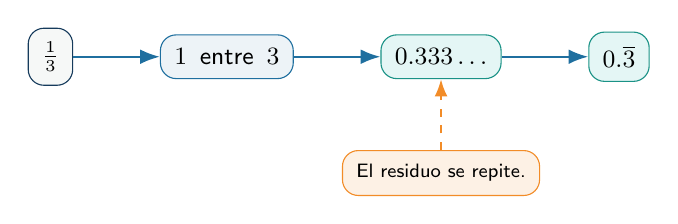
\begin{tikzpicture}[node distance=0.9cm and 1.1cm]
		\node[dato] (a) {$\frac{1}{3}$};
		\node[paso, right=of a] (b) {\DivOp{1}{3}};
		\node[resultado, right=of b] (c) {$0{.}333\ldots$};
		\node[resultado, right=of c] (d) {$0{.}\overline{3}$};
		\node[verificacion, below=of c] (e) {El residuo se repite.};
		\draw[flecha] (a) -- (b);
		\draw[flecha] (b) -- (c);
		\draw[flecha] (c) -- (d);
		\draw[flechaSecundaria] (e) -- (c);
	\end{tikzpicture}}
	\caption{Procedimiento visual para reconocer un decimal periódico.}
\end{figure}

\subsection{Números decimales finitos a fracción}

La tabla presenta varios incisos resueltos; el esquema posterior muestra la ruta de procedimiento que se aplica al bloque completo.

\begin{longtable}{@{}p{0.23\linewidth}p{0.23\linewidth}p{0.23\linewidth}p{0.23\linewidth}@{}}
	\caption{Conversión de números decimales finitos}\label{tab:decimales-finitos}\\
	\toprule
	\textbf{1--2} & \textbf{3--4} & \textbf{5--6} & \textbf{7--8} \\
	\midrule
	\endfirsthead
	\toprule
	\textbf{1--2} & \textbf{3--4} & \textbf{5--6} & \textbf{7--8} \\
	\midrule
	\endhead
	1. $1{.}6=\frac{8}{5}$ & 3. $0{.}025=\frac{1}{40}$ & 5. $34{.}5=\frac{69}{2}$ & 7. $0{.}17=\frac{17}{100}$ \\
	2. $0{.}525=\frac{21}{40}$ & 4. $0{.}75=\frac{3}{4}$ & 6. $1{.}5=\frac{3}{2}$ & 8. $2{.}05=\frac{41}{20}$ \\
	\bottomrule
\end{longtable}

\begin{figure}[H]
	\centering
	\resizebox{0.92\linewidth}{!}{%
		\ejercicioTikzTresPasos
			{$0{.}525$}
			{Quitar punto decimal}
			{$\frac{525}{1000}$}
			{$\frac{21}{40}$}
			{Tres cifras decimales $\Rightarrow$ denominador $1000$.}
	}
	\caption{Procedimiento visual para convertir un decimal finito a fracción.}
\end{figure}

\subsection{Números decimales periódicos a fracción}

La tabla presenta varios incisos resueltos; el esquema posterior muestra la ruta de procedimiento que se aplica al bloque completo.

\begin{longtable}{@{}p{0.23\linewidth}p{0.23\linewidth}p{0.23\linewidth}p{0.23\linewidth}@{}}
	\caption{Conversión de números decimales periódicos}\label{tab:decimales-periodicos}\\
	\toprule
	\textbf{1--2} & \textbf{3--4} & \textbf{5--6} & \textbf{7--8} \\
	\midrule
	\endfirsthead
	\toprule
	\textbf{1--2} & \textbf{3--4} & \textbf{5--6} & \textbf{7--8} \\
	\midrule
	\endhead
	1. $0{.}\overline{18}=\frac{2}{11}$ & 3. $2{.}1\overline{6}=\frac{13}{6}$ & 5. $0{.}82\overline{1}=\frac{739}{900}$ & 7. $0{.}\overline{009}=\frac{1}{111}$ \\
	2. $0{.}\overline{7}=\frac{7}{9}$ & 4. $0{.}5\overline{3}=\frac{8}{15}$ & 6. $1{.}4\overline{67}=\frac{1453}{990}$ & 8. $5{.}8\overline{72}=\frac{323}{55}$ \\
	\bottomrule
\end{longtable}

\begin{figure}[H]
	\centering
	\resizebox{0.76\linewidth}{!}{%
	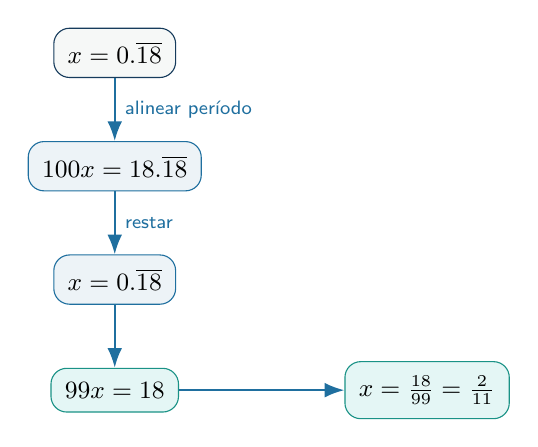
\begin{tikzpicture}[node distance=0.8cm]
		\node[dato] (x) {$x=0{.}\overline{18}$};
		\node[paso, below=of x] (a) {$100x=18{.}\overline{18}$};
		\node[paso, below=of a] (b) {$x=0{.}\overline{18}$};
		\node[resultado, below=of b] (c) {$99x=18$};
		\node[resultado, right=2.1cm of c] (d) {$x=\frac{18}{99}=\frac{2}{11}$};
		\draw[flecha] (x) -- node[right, font=\scriptsize] {alinear período} (a);
		\draw[flecha] (a) -- node[right, font=\scriptsize] {restar} (b);
		\draw[flecha] (b) -- (c);
		\draw[flecha] (c) -- (d);
	\end{tikzpicture}}
	\caption{Procedimiento visual para convertir un decimal periódico puro a fracción.}
\end{figure}

\section{Situaciones en contexto}

\begin{longtable}{@{}p{0.12\linewidth}p{0.48\linewidth}p{0.34\linewidth}@{}}
	\caption{Resolución de situaciones contextualizadas}\label{tab:situaciones}\\
	\toprule
	\textbf{Situación} & \textbf{Planteamiento} & \textbf{Respuesta} \\
	\midrule
	\endfirsthead
	\toprule
	\textbf{Situación} & \textbf{Planteamiento} & \textbf{Respuesta} \\
	\midrule
	\endhead
	01 & Rezago educativo: CDMX $9$ de cada $100$; Estado de México y Coahuila $14$ de cada $100$; Chiapas $32$ de cada $100$; Oaxaca y Michoacán $29$ de cada $100$. & CDMX $0{.}09$; Estado de México y Coahuila $0{.}14$; Chiapas $0{.}32$; Oaxaca y Michoacán $0{.}29$. \\
	02 & Edad del hermano de Rosalinda: $4\frac{5}{12}$ años. & $4\frac{5}{12}=\frac{53}{12}=4{.}41\overline{6}$ años. \\
	03 & Eduardo sembró $7$ de $18$ partes de su parcela; expresar lo que falta. & Falta $\frac{11}{18}=0{.}6\overline{1}$. \\
	04 & El IVA es $0{.}16$; expresar como fracción común. & $0{.}16=\frac{16}{100}=\frac{4}{25}$. \\
	05 & Un galón equivale a $3{.}790$ litros; expresar como fracción simplificada. & $3{.}790=\frac{3790}{1000}=\frac{379}{100}$. \\
	06 & Una llave española mide $\frac{11}{16}$ pulgadas. & $\frac{11}{16}=0{.}6875$ pulgadas. \\
	07 & Expresar las medidas mostradas como fracciones decimales. & Usar lectura decimal y escribirla con denominador $10$, $100$ o $1000$, según sus cifras decimales. \\
	08 & Identificar la fracción correspondiente al peso mostrado en la báscula. & Leer el valor de la escala y expresarlo como fracción de la unidad indicada. \\
	09 & Felipe requiere un hilo de $\frac{7}{40}$ mm y los catálogos están en decimal. & $\frac{7}{40}=0{.}175$ mm. \\
	10 & Calcular el perímetro del cuadrilátero y expresarlo como fracción simplificada. & Sumar las cuatro medidas de la figura y simplificar la fracción resultante. \\
	11 & Representar en decimal los diámetros de las ruedas. & Dividir numerador entre denominador en cada diámetro mostrado. \\
	12 & Calcular el perímetro del rectángulo y expresarlo como número decimal. & Usar $P=2(largo+ancho)$ y convertir el resultado a decimal. \\
	\bottomrule
\end{longtable}

\subsection{Esquemas de apoyo para situaciones en contexto}

Las siguientes representaciones muestran el procedimiento matemático que debe seguirse en situaciones de medición, peso, perímetro y diámetro. El objetivo es identificar el dato numérico, traducirlo a fracción o decimal y verificar que el resultado conserve la magnitud original.

\begin{figure}[H]
	\centering
	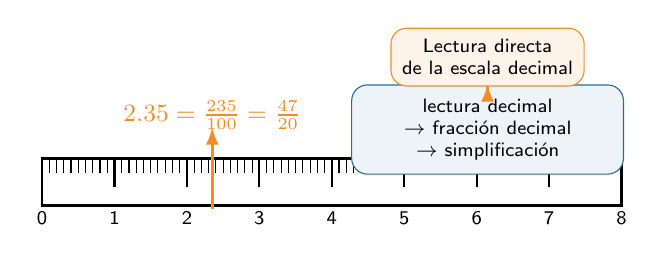
\begin{tikzpicture}[scale=0.92]
		\draw[thick] (0,0) rectangle (8,0.65);
		\foreach \x in {0,...,8}{
			\draw[thick] (\x,0.65) -- (\x,0.25);
			\node[font=\scriptsize] at (\x,-0.18) {\x};
		}
		\foreach \x in {0.1,0.2,...,7.9}{\draw (\x,0.65) -- (\x,0.45);}
		\draw[iiiepeOrange, very thick] (2.35,0.9) -- (2.35,-0.05);
		\draw[flechaSecundaria] (2.35,0.9) -- (2.35,1.08);
		\node[font=\small, color=iiiepeOrange] at (2.35,1.25) {$2.35=\frac{235}{100}=\frac{47}{20}$};
		\node[paso, text width=3.1cm, align=center, font=\scriptsize] (rutaEscala) at (6.15,1.05) {lectura decimal\\$\rightarrow$ fracción decimal\\$\rightarrow$ simplificación};
		\node[nota] (lecturaEscala) at (6.15,2.05) {Lectura directa\\de la escala decimal};
		\draw[flechaSecundaria] (lecturaEscala.south) -- (rutaEscala.north);
	\end{tikzpicture}
	\caption{Situación 07: lectura de una medida decimal y conversión a fracción decimal.}
\end{figure}

\begin{figure}[H]
	\centering
	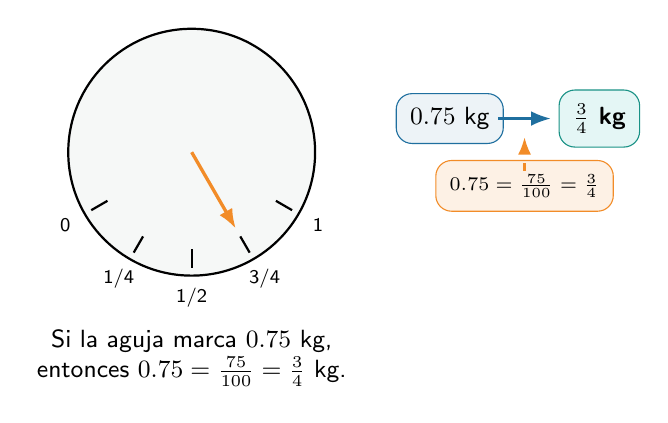
\begin{tikzpicture}[scale=0.95]
		\draw[thick, fill=iiiepePaper] (0,0) circle (1.65);
		\foreach \ang/\lab in {210/0,240/{1/4},270/{1/2},300/{3/4},330/1}{
			\draw[thick] (\ang:1.30) -- (\ang:1.55);
			\node[font=\scriptsize] at (\ang:1.95) {\lab};
		}
		\draw[iiiepeOrange, very thick, -{Latex[length=2.5mm]}] (0,0) -- (300:1.18);
		\node[font=\small, align=center] at (0,-2.75) {Si la aguja marca $0{.}75$ kg,\\entonces $0{.}75=\frac{75}{100}=\frac{3}{4}$ kg.};
		\node[paso] at (3.45,0.45) {$0{.}75$ kg};
		\node[resultado] at (5.45,0.45) {$\frac{3}{4}$ kg};
		\node[verificacion] at (4.45,-0.45) {$0{.}75=\frac{75}{100}=\frac{3}{4}$};
		\draw[flecha] (4.10,0.45) -- (4.80,0.45);
		\draw[flechaSecundaria] (4.45,-0.25) -- (4.45,0.20);
	\end{tikzpicture}
	\caption{Situación 08: lectura de báscula como fracción de la unidad.}
\end{figure}

\begin{figure}[H]
	\centering
	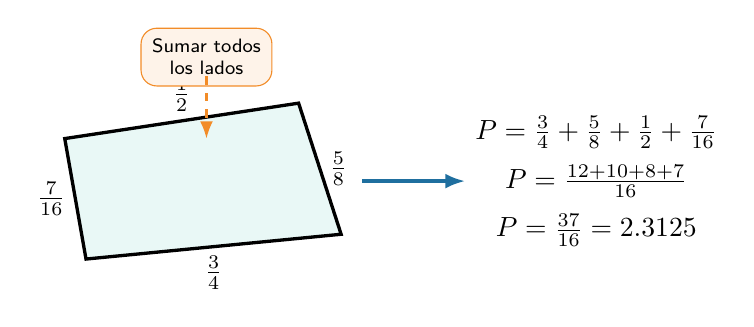
\begin{tikzpicture}[scale=0.9]
		\coordinate (A) at (0,0);
		\coordinate (B) at (3.6,0.35);
		\coordinate (C) at (3.0,2.2);
		\coordinate (D) at (-0.30,1.7);
		\draw[very thick, fill=iiiepeAqua!10] (A)--(B)--(C)--(D)--cycle;
		\node[below] at ($(A)!0.5!(B)$) {$\frac{3}{4}$};
		\node[right] at ($(B)!0.5!(C)$) {$\frac{5}{8}$};
		\node[above] at ($(C)!0.5!(D)$) {$\frac{1}{2}$};
		\node[left] at ($(D)!0.5!(A)$) {$\frac{7}{16}$};
		\node[nota] at (1.7,2.85) {Sumar todos\\los lados};
		\draw[flechaSecundaria] (1.7,2.58) -- (1.7,1.70);
		\node[align=center] at (7.2,1.1) {
			$P=\frac{3}{4}+\frac{5}{8}+\frac{1}{2}+\frac{7}{16}$\\[2mm]
			$P=\frac{12+10+8+7}{16}$\\[2mm]
			$P=\frac{37}{16}=2{.}3125$
		};
		\draw[-{Latex[length=2.5mm]}, very thick, iiiepeBlue] (3.9,1.1) -- (5.35,1.1);
	\end{tikzpicture}
	\caption{Situación 10: procedimiento para calcular perímetro con fracciones.}
\end{figure}

\begin{figure}[H]
	\centering
	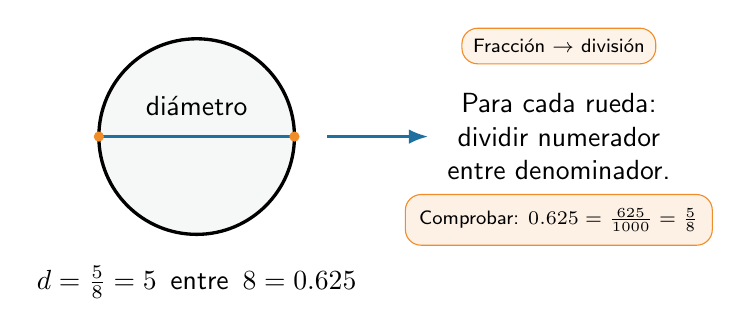
\begin{tikzpicture}[scale=0.92]
		\draw[very thick, fill=iiiepePaper] (0,0) circle (1.35);
		\draw[very thick, iiiepeBlue] (-1.35,0) -- (1.35,0);
		\fill[iiiepeOrange] (-1.35,0) circle (2pt);
		\fill[iiiepeOrange] (1.35,0) circle (2pt);
		\node[above] at (0,0.15) {diámetro};
		\node[below] at (0,-1.65) {$d=\frac{5}{8}=\DivOp{5}{8}=0{.}625$};
		\node[align=center] at (5.0,0) {Para cada rueda:\\ dividir numerador\\ entre denominador.};
		\node[nota] at (5.0,1.25) {Fracción $\rightarrow$ división};
		\node[verificacion] at (5.0,-1.15) {Comprobar: $0{.}625=\frac{625}{1000}=\frac{5}{8}$};
		\draw[-{Latex[length=2.5mm]}, very thick, iiiepeBlue] (1.8,0) -- (3.2,0);
	\end{tikzpicture}
	\caption{Situación 11: conversión del diámetro fraccionario a decimal.}
\end{figure}

\begin{figure}[H]
	\centering
	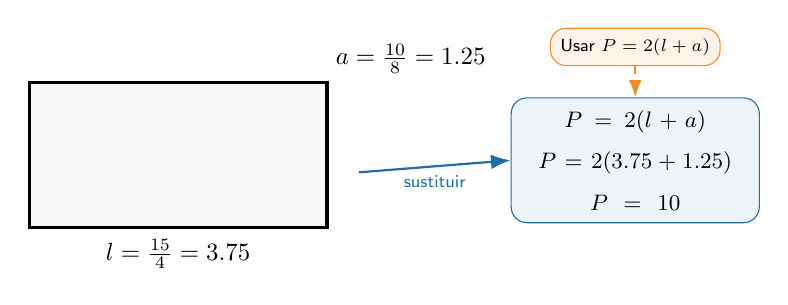
\begin{tikzpicture}[scale=0.9, transform shape]
		\draw[very thick, fill=iiiepePaper] (0,0) rectangle (4.2,2.05);
		\node[below] at (2.1,-0.04) {$l=\frac{15}{4}=3{.}75$};
		\node[above right] at (4.2,2.05) {$a=\frac{10}{8}=1{.}25$};
		\node[paso, text width=3.15cm, align=center] (desarrollo) at (8.55,0.95) {
			$P=2(l+a)$\\[2mm]
			$P=2(3{.}75+1{.}25)$\\[2mm]
			$P=10$
		};
		\node[nota] (regla) at (8.55,2.55) {Usar $P=2(l+a)$};
		\draw[flechaSecundaria] (regla.south) -- (desarrollo.north);
		\draw[flecha] (4.65,0.78) -- node[below, font=\scriptsize] {sustituir} (desarrollo.west);
	\end{tikzpicture}
	\caption{Situación 12: perímetro de rectángulo expresado en decimal.}
\end{figure}

\section{Evaluación y retroalimentación}

\subsection{Autoevaluación del estudiante}

\begin{table}[H]
\centering
\caption{Autoevaluación mejorada de la actividad}
\label{tab:autoevaluacion}

\small
\renewcommand{\arraystretch}{1.45}
\setlength{\tabcolsep}{5pt}
\rowcolors{2}{gray!10}{white}

\begin{tabularx}{\textwidth}{@{}
>{\raggedright\arraybackslash}X
>{\centering\arraybackslash}p{0.12\textwidth}
>{\centering\arraybackslash}p{0.14\textwidth}
>{\centering\arraybackslash}p{0.14\textwidth}
>{\centering\arraybackslash}p{0.07\textwidth}
@{}}
\toprule
\textbf{Indicador} &
\makecell{\textbf{Logrado}\\\textbf{(3)}} &
\makecell{\textbf{En proceso}\\\textbf{(2)}} &
\makecell{\textbf{No logrado}\\\textbf{(1)}} &
\textbf{Valor} \\
\midrule

Convierto fracciones a decimales de manera eficiente utilizando el algoritmo aprendido.
& $\square$ & $\square$ & $\square$ & \\

Convierto decimales finitos y periódicos a fracciones utilizando correctamente el procedimiento aprendido.
& $\square$ & $\square$ & $\square$ & \\

Reconozco y escribo decimales periódicos usando la notación correspondiente.
& $\square$ & $\square$ & $\square$ & \\

Selecciono la estrategia adecuada: valor posicional, división o eliminación del período.
& $\square$ & $\square$ & $\square$ & \\

Compruebo que la fracción y el decimal representan la misma cantidad.
& $\square$ & $\square$ & $\square$ & \\

Interpreto el resultado según el contexto del problema.
& $\square$ & $\square$ & $\square$ & \\

\bottomrule
\end{tabularx}

\end{table}

\subsection{Criterios para retroalimentar}

\begin{itemize}
	\item Si el estudiante divide denominador entre numerador, se recupera el significado de fracción como reparto: $\frac{a}{b}$ significa \DivOp{a}{b}.
	\item Si coloca mal el punto decimal en fracciones decimales, se revisa el valor posicional y el número de ceros del denominador.
	\item Si escribe un decimal periódico sin barra, se solicita identificar el bloque que se repite y verificarlo con los residuos de la división.
	\item Si convierte un decimal finito a fracción pero no simplifica, se revisa el máximo común divisor entre numerador y denominador.
	\item Si obtiene una respuesta correcta sin explicación, se pide agregar estrategia, desarrollo, resultado y comprobación.
\end{itemize}

% ==============================================================================
% SECCIÓN 4: CONCLUSIÓN
% Cierre recomendado:
% - Responder directamente a la actividad.
% - Indicar que se comprendió, no solo que se elaboró.
% - Mencionar criterio personal final.
% - No introducir información nueva.
% ==============================================================================
\section{Conclusión}

La mejora de la actividad permite comprobar que fracciones y decimales son formas equivalentes de representar números racionales, pero también que esa equivalencia debe demostrarse. Las fracciones decimales se convierten mediante valor posicional; las fracciones no decimales se convierten mediante división; y los decimales finitos o periódicos pueden expresarse como fracciones simplificadas.

El aprendizaje central es reconocer que la conversión no cambia la cantidad representada, solo cambia su escritura. Por ello, cada resultado debe verificarse con el procedimiento correspondiente, con la simplificación adecuada y con el sentido del contexto en que se utiliza.

La retroalimentación incorporada desde la Sesión 02 fortalece el producto porque convierte la actividad en una secuencia didáctica completa: recupera antecedentes, explica procedimientos, propone práctica graduada, evalúa en contexto y cierra con criterios concretos de mejora.
% FIN DEL DOCUMENTO
\end{document}
